\section{Desenvolvimento}

% Slide 2: Estrutura de Pacotes
\begin{frame}{Desenvolvimento - Arquitetura do Compilador}
    \begin{itemize}
        \item Organização modular para encapsulamento de responsabilidades:
        \begin{itemize}
            \item \texttt{lexer}: Análise léxica e tokenização.
            \item \texttt{parser}: Construção da AST com \textit{Pratt Parsing}.
            \item \texttt{walker}: Navegação e análise da AST.
            \item \texttt{checker}: Inferência de tipos e validações semânticas.
            \item \texttt{emitter}: Geração do código GLSL.
        \end{itemize}
    \end{itemize}
    \begin{figure}
        \centering
        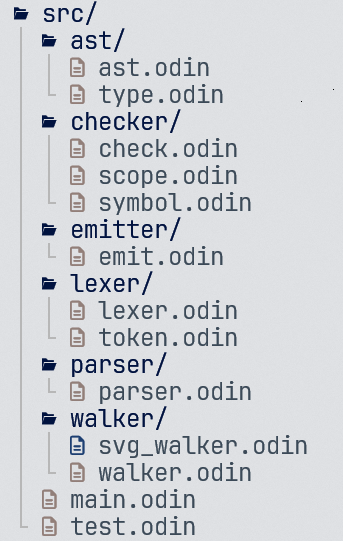
\includegraphics[scale=0.34]{./Imagens/package-structure.png}
        \caption{\small Estrutura de pacotes do compilador.}
    \end{figure}
\end{frame}


\begin{frame}{Arquitetura do Compilador}
    \begin{figure}
        \centering
        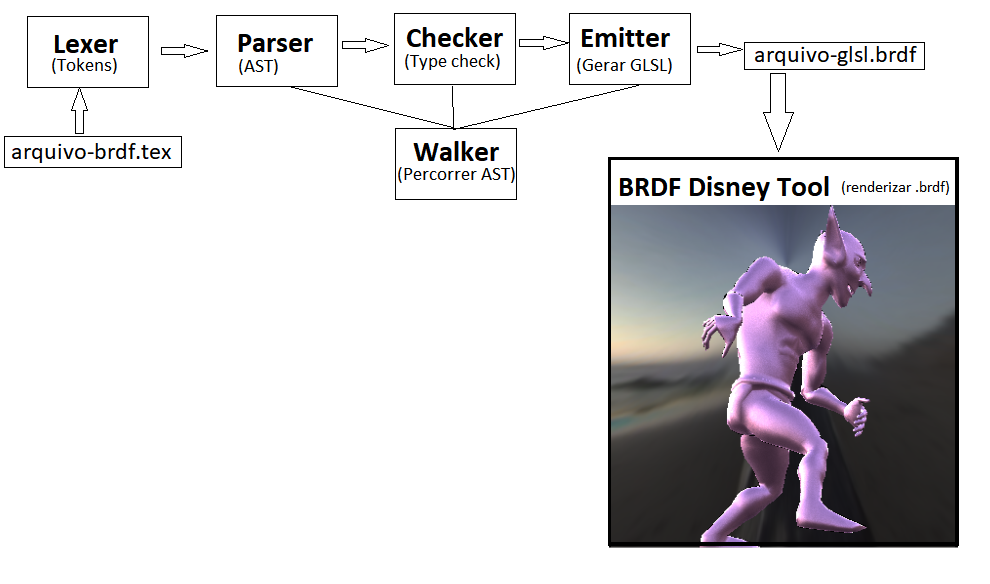
\includegraphics[scale=0.35]{./Imagens/estutura-geral-do-projeto.png}
        \caption{\small Estrutura geral da arquitetura do compilador.}
    \end{figure}
\end{frame}

\begin{frame}{Destaques do Desenvolvimento}
    \begin{itemize}
        \item Análise sintática baseada em \textit{Pratt Parsing}, garantindo precisão e hierarquia nas expressões.
        \item Funcionalidades do \texttt{walker}:
        \begin{itemize}
            \item Navegação genérica e preparação para verificações.
            \item Suporte uniforme à travessia de nós.
        \end{itemize}
        \item Integração do \texttt{checker} com a tabela de símbolos para validações semânticas e consistência.
        \item Geração de \textit{shaders} GLSL compatíveis com Disney BRDF Explorer.
    \end{itemize}
\end{frame}

